\section{Introduction}

In the day-to-day life our head scatters how the sound arrives to our ears making it easier to deduce if the sound comes from our right because we would be able to hear better the sound in our right ear than in the left one and vice-versa. Simultaneously this scattering has also a different interest. Indeed, people who lost their hearing in one ear use this scattering to help them deduce where the sound they're hearing comes from, notably by using the power of the sound i.e. if the sound seems loud it probably comes from their hearing side and alternatively if it seems soft it probably comes from their non-hearing side.

This functionality to use its head as a way to deduce the direction of arrival of a sound is relative to what is called the head-related transfer function (HRTF) in humans and other animals. But the head scattering is, of course, not the only scattering possible to be able to deduce the direction of arrival with only one receiver. Indeed some recent work has shown that, while using a microphone surrounded by LEGO\textsuperscript{\textcopyright} bricks, it was possible to have an estimation of the direction of arrival \cite{dalia}. However in this project we will try to have a generalization of this concept and use a scattering with several microphones and not just one to see if it helps.

The goal of this project is to compare various localization algorithms with and without the presence of scattering. The different impulse response we would use are :
\begin{itemize}
    \item A LEGO response impulse : in this response we have 6 microphones at different positions. We can see the positions of the LEGOs and the ones of the microphones in figure \ref{fig:lego} (2 of the microphones are not really visible because they are under the yellow truck).
    \item A KEMAR response impulse : a device simulating a human head and torso visible at figure \ref{fig:kemar}. In this response we have 2 microphones that simulates the ears of a human.
    \item An omnidirectional response impulse : an analytically computed response to simulate an omnidirectional microphone receiver that has nothing around him.
\end{itemize}

\begin{figure}[h]
\centering
\begin{minipage}{.5\textwidth}
    \caption{LEGO\textsuperscript{\textcopyright} and microphones disposition}
    \centering
    \label{fig:lego}
    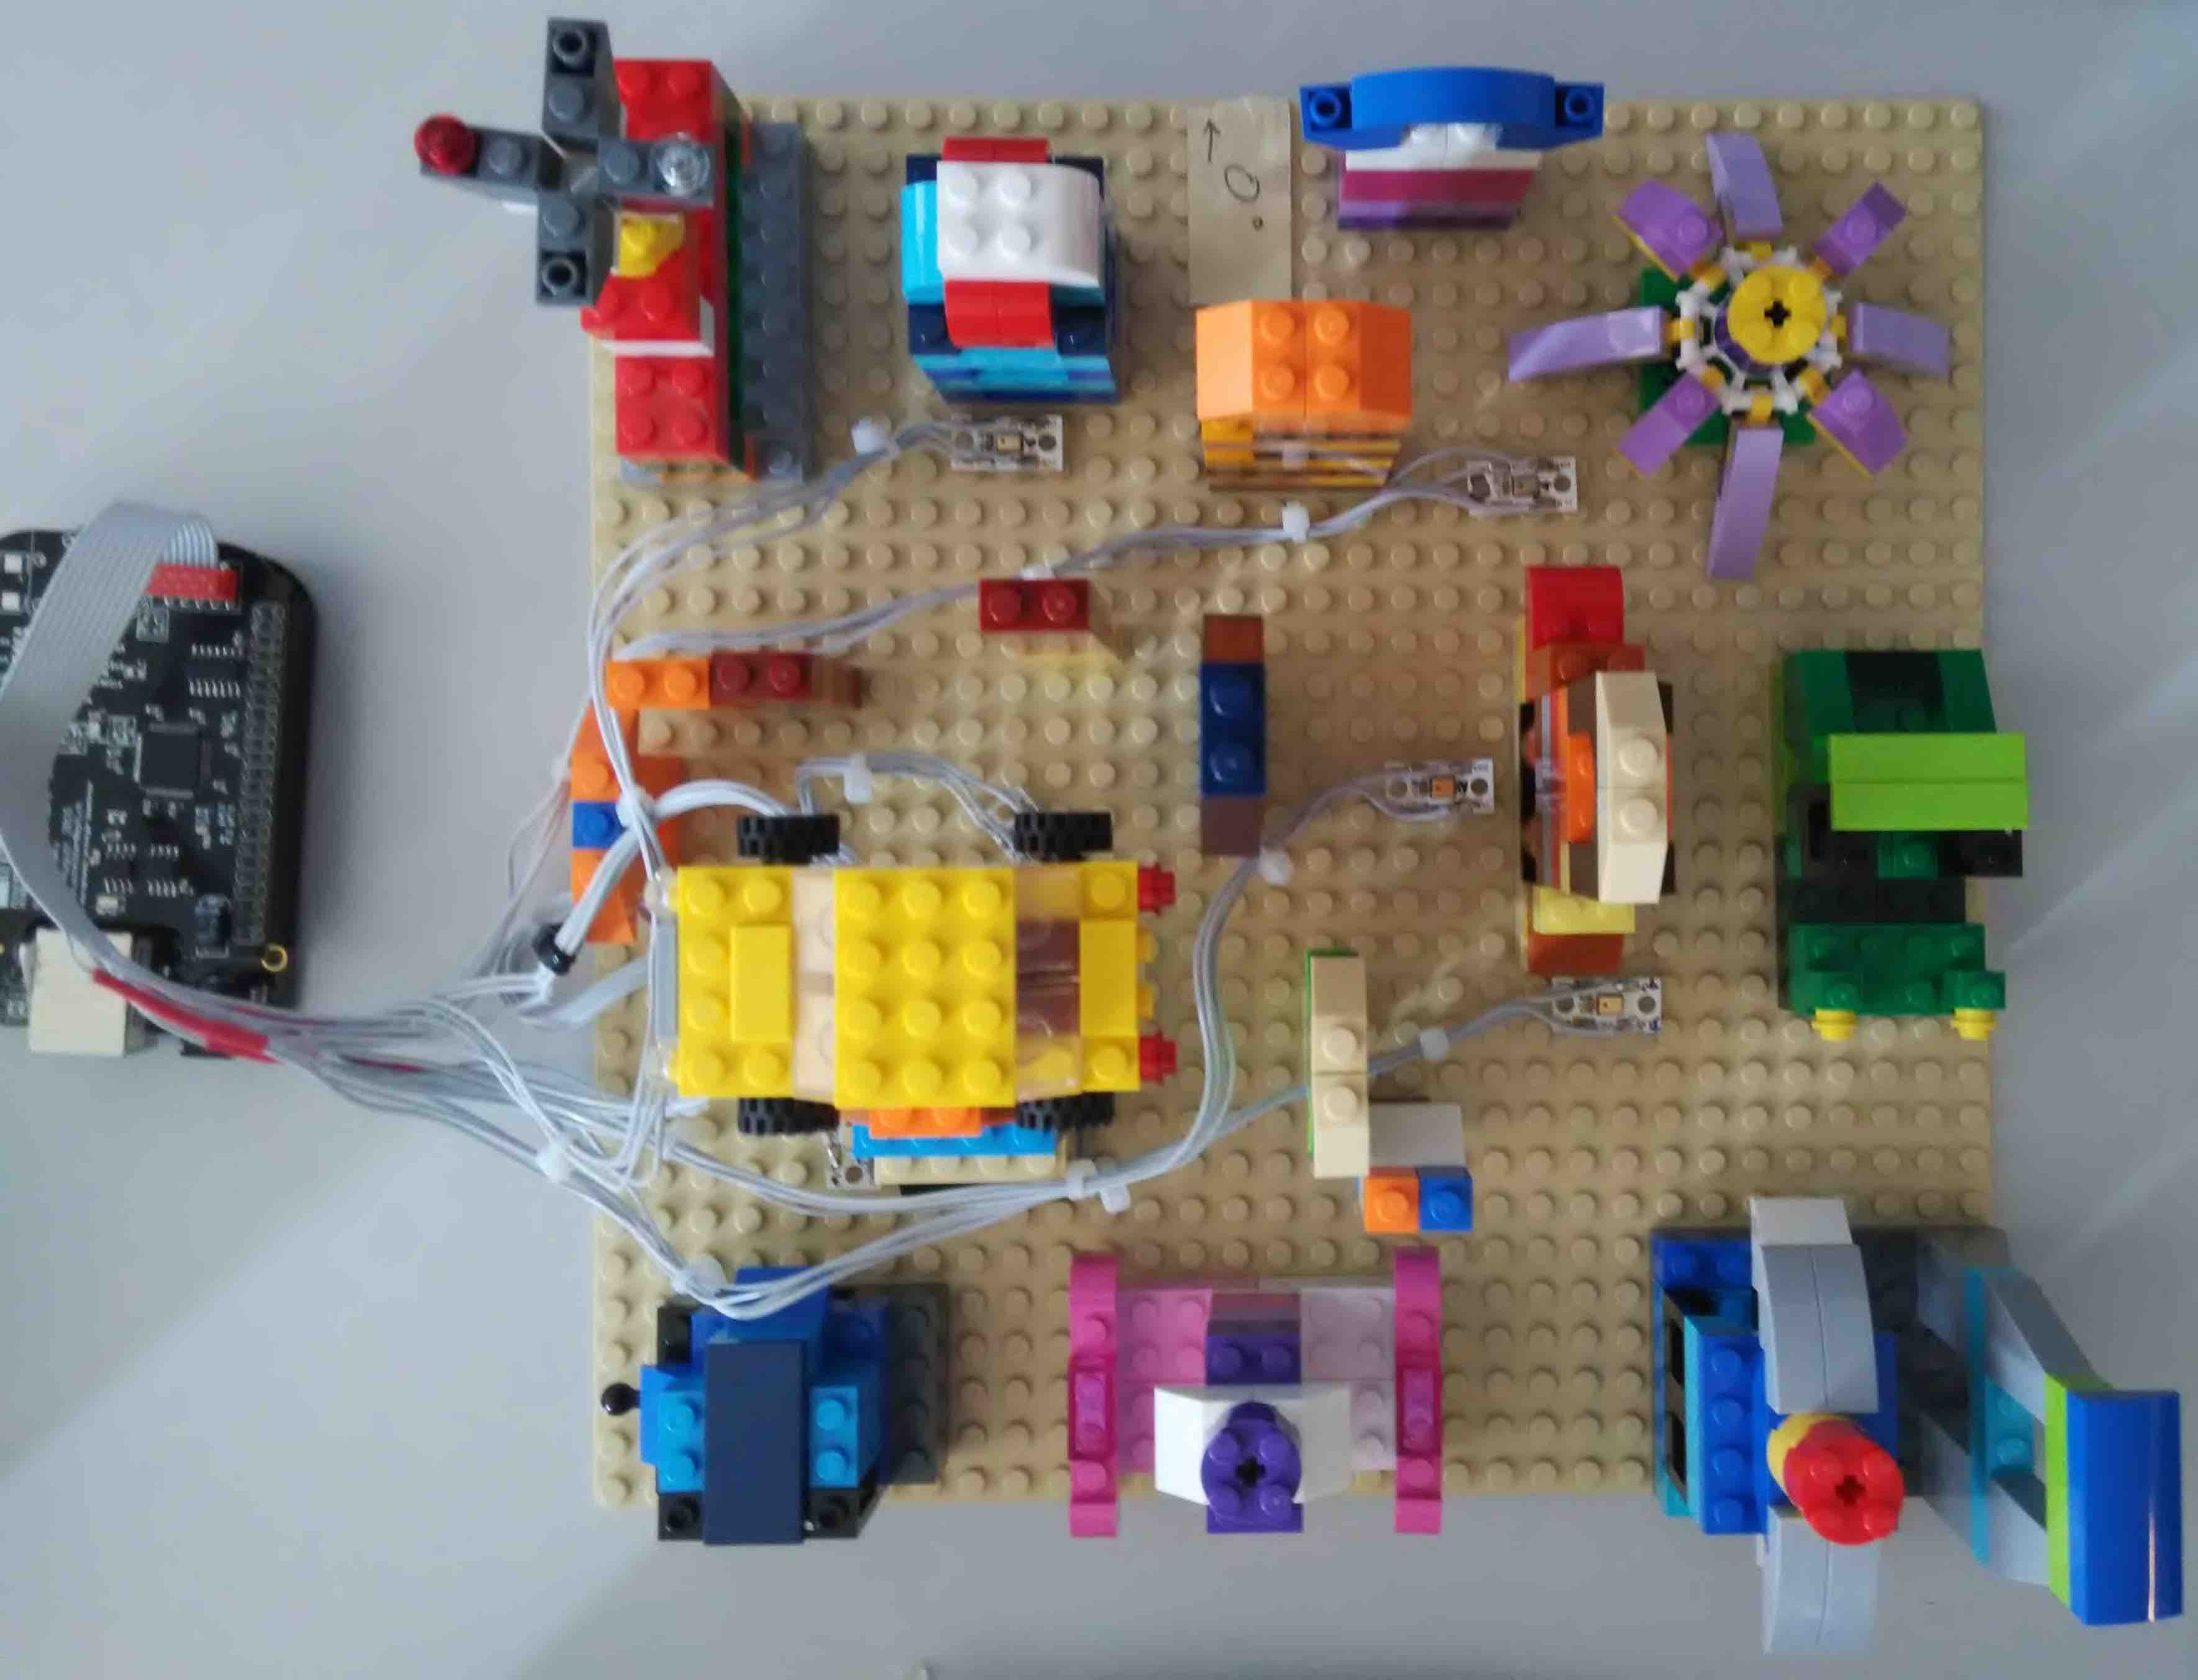
\includegraphics[width=0.8\textwidth]{lego_top.jpg}
\end{minipage}%
\begin{minipage}{.5\textwidth}
    \caption{KEMAR head and torso simulator}
    \centering
    \label{fig:kemar}
    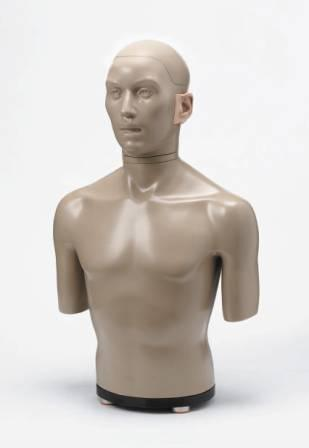
\includegraphics[width=0.5\textwidth]{Kemar.jpeg}
\end{minipage}
\end{figure}